% Python debugging
% by Roman gryf Dobosz 2015

% \documentclass[14pt,notes,svgnames,aspectratio=1610]{beamer}
\documentclass[14pt,notes,svgnames,aspectratio=169]{beamer}
% \documentclass[14pt,notes,svgnames]{beamer}
\usecolortheme{seagull}

\usecolortheme[RGB={23,57,107}]{structure}
\usenavigationsymbolstemplate{}  % Gets rid of slide navigation symbols
\usefonttheme{professionalfonts} % using non standard fonts for beamer

% for proper underline
\usepackage[normalem]{ulem}

\usepackage{fontspec}
\defaultfontfeatures{Ligatures=TeX}

% color and font customization
\definecolor{ExecusharesEmph}{RGB}{20,57,107}
\definecolor{ExecusharesBlack}{RGB}{47,42,42}
\definecolor{ExecusharesWhite}{RGB}{211,205,193}
\definecolor{ExecusharesGrey}{RGB}{96,83,58}

\setmainfont{Helvetica Neue}
\setsansfont{Helvetica Neue}
\setmonofont{DejaVu Sans Mono}

\setbeamercolor{itemize item}{fg=ExecusharesEmph}
\setbeamercolor{enumerate item}{fg=ExecusharesEmph}
\setbeamercolor{alerted text}{fg=ExecusharesEmph}
\setbeamercolor{section in toc}{fg=ExecusharesBlack}

\setbeamercolor{background canvas}{bg=ExecusharesWhite}
\setbeamercolor{normal text}{fg=ExecusharesEmph}

\setbeamerfont{author}{size*={14}{1.4em}}
\setbeamerfont{date}{size*={7}{0.7em}}

\useinnertheme{circles}

\usepackage{graphicx}
% \usepackage{sidecap}
% \usepackage{hyperref}

\usepackage{listings}


\definecolor{ListingsKeywords}{RGB}{107,81,42}
\definecolor{ListingsComments}{RGB}{20,56,107}
\definecolor{ListingsStrings}{RGB}{90,20,107}
\definecolor{ListingsIdentifiers}{RGB}{39,107,20}

\lstset{language=Python,
    basicstyle=\ttfamily\small,
    keywordstyle=\color{ListingsKeywords},
    commentstyle=\color{ListingsComments},
    stringstyle=\color{ListingsStrings},
    showstringspaces=false,
    identifierstyle=\color{ListingsIdentifiers}
}

\setbeamerfont{framesubtitle}{family=\fontfamily{hvt}\selectfont}

\setbeamerfont{frametitle}{series=\bfseries}

\setbeamertemplate{frametitle}{%
    \begin{centering}
        \textbf{\insertframetitle}
        \par
    \end{centering}
}

\setbeamertemplate{custom section}
{%
    \begin{centering}
        \usebeamerfont{section title}
        \Large\bfseries
        {\color{ExecusharesWhite}\insertsection\par}
    \end{centering}
}
\def\sectionpage{\usebeamertemplate*{custom section}}

\defbeamertemplate*{title page}{customized}[1][]
{%
    \center
    \usebeamerfont{title}\inserttitle\par
    \bigskip
    {\color{ExecusharesEmph} \usebeamerfont{author}\insertauthor\par}
    \usebeamerfont{institute}\insertinstitute\par
    \bigskip
    \usebeamerfont{date}\insertdate\par
}

\AtBeginSection{\frame{\sectionpage}}

\begin{document}

\title{%
    
\includegraphics[width=7cm]{images/title.pdf}
}
\author{Roman Dobosz}
\date{PyGDA, 29 June, 2015}

\begin{frame}
  \titlepage
\end{frame}

\begingroup
    \setbeamercolor{background canvas}{bg=ExecusharesBlack}
    \section{Agenda}
\endgroup

\begin{frame}
    \begin{columns}
        \column{.5\textwidth}
        \begin{itemize}[<+->]
            \item<1,2,3> Failure detection
            \item<2,3> Python debuggers
            \item<3> \lstinline{pdb} in practice
        \end{itemize}
        \column{.4\textwidth}
        \centering
        \only<1>{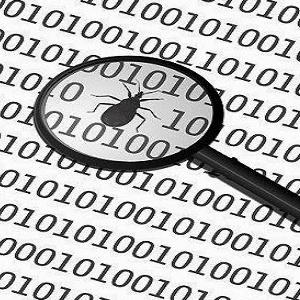
\includegraphics[width=3cm]{images/find_bug.png}}
        \only<2>{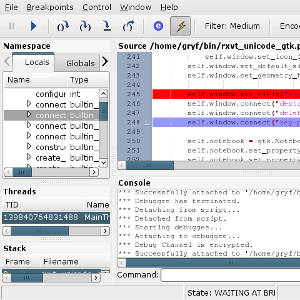
\includegraphics[width=3cm]{images/debugs.png}}
        \only<3>{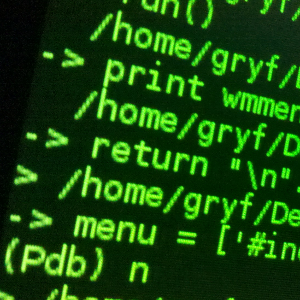
\includegraphics[width=3cm]{images/pdb.png}}
    \end{columns}
\end{frame}

\begingroup
    \setbeamercolor{background canvas}{bg=ExecusharesBlack}
    \section{How to find the place of a failure}
\endgroup

\begin{frame}
    \begin{columns}
        \column{.5\textwidth}
        \begin{itemize}[<+->]
            \item<1,2,3,4,5> traceback (obviously)
            \item<2,3,4,5> \lstinline{print} statement
            \item<3,4,5> module \lstinline{logging}
            \item<4,5> module \lstinline{trace}
            \item<5> debugger
        \end{itemize}
        \column{.4\textwidth}
        \centering
        \only<1>{%
            \vspace*{0cm}
            \hspace*{0cm}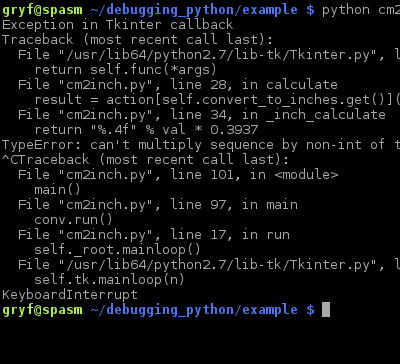
\includegraphics[width=5cm]{images/traceback.png}
        }
        \only<2>{%
            \vspace*{0cm}
            \hspace*{0cm}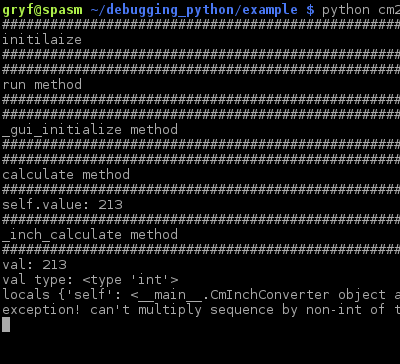
\includegraphics[width=5cm]{images/print.png}
        }
        \only<3>{%
            \vspace*{0cm}
            \hspace*{0cm}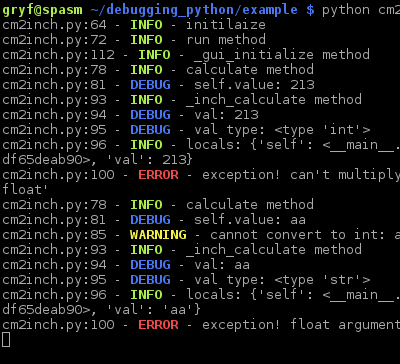
\includegraphics[width=5cm]{images/logging.png}
        }
        \only<4>{%
            \vspace*{0cm}
            \hspace*{0cm}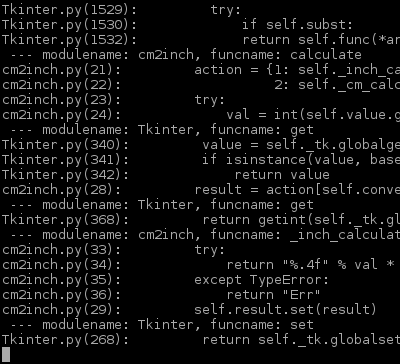
\includegraphics[width=5cm]{images/trace.png}
        }
        \only<5>{%
            \vspace*{0cm}
            \hspace*{0cm}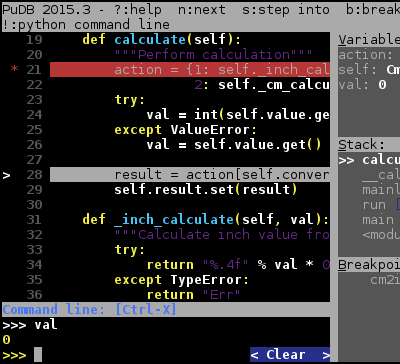
\includegraphics[width=5cm]{images/pudb.png}
        }
    \end{columns}
\end{frame}

\begingroup
    \setbeamercolor{background canvas}{bg=ExecusharesBlack}
    \section{Python debuggers}
\endgroup

\begin{frame}
    Debuggers can be divided in several different aspects

    \begin{columns}
        \column{.5\textwidth}
        \begin{itemize}[<+->]
            \item<1,2,3> Text based
            \item<2,3> Graphical
            \item<3> Embedded in IDE
        \end{itemize}
        \column{.4\textwidth}
    \end{columns}
\end{frame}

\begin{frame}
    \frametitle{Debuggers - text based}
    \begin{columns}
        \column{.4\textwidth}
        \begin{itemize}
            \item \lstinline{pdb}
            \item \lstinline{ipdb}
            \item \lstinline{pdb++}
            \item \lstinline{pudb}
            \item \color{blue}\href{https://wiki.python.org/moin/PythonDebuggingTools}{\uline{others}}
        \end{itemize}
        \column{.5\textwidth}

        \vspace*{0cm}
        \hspace*{0cm}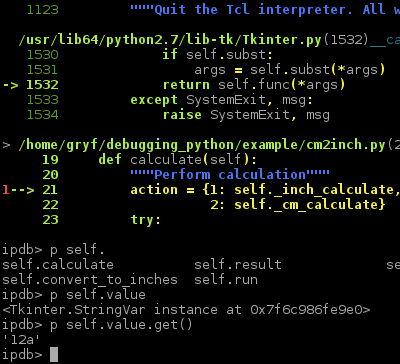
\includegraphics[width=5cm]{"images/ipdb.png"}

    \end{columns}
\end{frame}

\begin{frame}
    \frametitle{Debuggers - graphical}
    \begin{columns}
        \column{.4\textwidth}
        \begin{itemize}
            \item Winpdb
            \item \lstinline{pywin.debugger}
        \end{itemize}
        \column{.5\textwidth}

        \vspace*{0cm}
        \hspace*{0cm}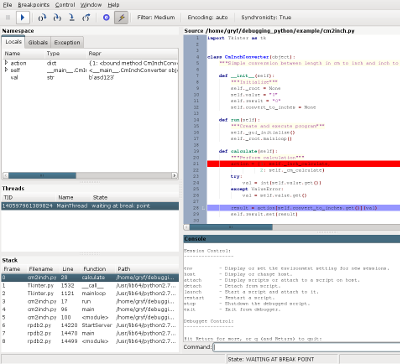
\includegraphics[width=5cm]{"images/winpdb.png"}

    \end{columns}
\end{frame}

\begin{frame}
    \frametitle{Debuggers - IDE}
    \begin{columns}
        \column{.4\textwidth}
        \begin{itemize}
            \item PyCharm
            \item PyDev (Eclipse)
            \item Wings IDE
            \item Visual Studio
            \item \color{blue}\href{https://wiki.python.org/moin/IntegratedDevelopmentEnvironments}{\uline{others!}}
        \end{itemize}
        \column{.5\textwidth}

        \vspace*{0cm}
        \hspace*{0cm}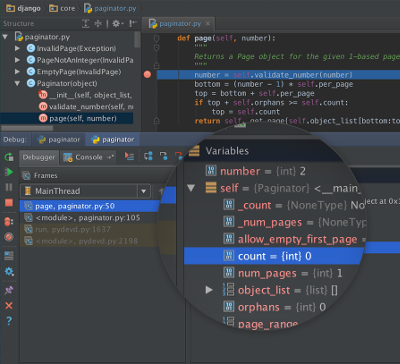
\includegraphics[width=5cm]{"images/pycharm.png"}

    \end{columns}
\end{frame}

\begingroup
    \setbeamercolor{background canvas}{bg=ExecusharesBlack}
    \section{Python debugger - pdb}
\endgroup

\begin{frame}
    \frametitle{cm2inch.py}
    \begin{itemize}
        \item Problem: Convert length in centimetre into inch and vice versa
        \item Solution: Simple TKinter program to do this
        \pause
        \item …But it doesn't work :(
    \end{itemize}
\end{frame}

\begin{frame}
    \frametitle{cm2inch.py - structure}
    \begin{itemize}
        \item Single class defined - \lstinline{CmInchConverter}
        \item Method \lstinline{run} launches the program
        \item Method \lstinline{_gui_initialze} builds the GUI
        \item Method \lstinline{calculate} implements the actual calculation logic
    \end{itemize}
\end{frame}

\begin{frame}
    \centerline{\Large Let see it in action!}
\end{frame}

\begingroup
    \setbeamercolor{background canvas}{bg=ExecusharesBlack}
    \section{Questions?}
\endgroup

\begin{frame}
    \centerline{\Large Thank you!}
\end{frame}

\end{document}
